\documentclass{article}

% Symbols
\usepackage[T1]{fontenc}
\usepackage{upgreek}
\usepackage{physics}
\usepackage{cancel}
\usepackage{amsfonts, amsthm}
\usepackage{amssymb, latexsym, amsmath}

%Algorithms
\usepackage[ruled,lined,linesnumbered,commentsnumbered]{algorithm2e}

%% Identación
\setlength{\parindent}{0cm}

%% Matrices
\usepackage{amssymb}
\usepackage{amsmath}
\usepackage{amsthm}

% Código
\newcommand{\code}[1]{\textcolor{white!25!black}{\texttt{#1}}}
\usepackage{listings}

%AMS
\usepackage{amsthm}
\newtheorem{algo-thm}{Algoritmo}

% Proof
\renewcommand*{\proofname}{\textbf{Demostraci\'on:}}
% Theorem
\newtheorem*{theorem}{Teorema}

% Graphics
\usepackage{graphicx}
\usepackage{pgf}

% Color a letras.
%\usepackage[usenames,dvipsnames,svgnames,table]{xcolor}

% Tikz
\usepackage{tkz-graph}
\usepackage{tikz}
\usetikzlibrary{arrows,automata}
\usepackage{tikz}
\usetikzlibrary{arrows,automata}
%\usetikzlibrary[topaths]

% Def. Dr. César.
\usetikzlibrary{shapes,calc}
\tikzstyle{edge}=[shorten <=2pt, shorten >=2pt, >=stealth, line width=1.1pt]
\tikzstyle{blueE}=[shorten <=2pt, shorten >=2pt, >=stealth, line width=1.5pt, blue]
\tikzstyle{blackV}=[circle, fill=black, minimum size=6pt, inner sep=0pt, outer sep=0pt]
\tikzstyle{blueV}=[circle, fill=blue, draw, minimum size=6pt, line width=0.75pt, inner sep=0pt, outer sep=0pt]
\tikzstyle{redV}=[circle, fill=red, draw, minimum size=6pt, line width=0.75pt, inner sep=0pt, outer sep=0pt]
\tikzstyle{redSV}=[semicircle, fill=red, minimum size=3pt, inner sep=0pt, outer sep=0pt, rotate=225]
\tikzstyle{blueSV}=[semicircle, fill=blue, minimum size=3pt, inner sep=0pt, outer sep=0pt, rotate=225]
\tikzstyle{blackSV}=[semicircle, fill=black, minimum size=3pt, inner sep=0pt, outer sep=0pt, rotate=225]
\tikzstyle{vertex}=[circle, draw, minimum size=6pt, line width=0.75pt, inner sep=0pt, outer sep=0pt]

% Margins
\addtolength{\voffset}{-1.5cm}
\addtolength{\hoffset}{-1.5cm}
\addtolength{\textwidth}{3cm}
\addtolength{\textheight}{3cm}

%Header-Footer
\usepackage{fancyhdr}
\renewcommand{\headrulewidth}{1pt}

\newcommand{\set}[1]{
  \left\{ #1 \right\}
}

%\pagenumbering{gobble} -- Este comando
%                       -- quita el número de página.
\footskip = 50pt
\renewcommand{\headrulewidth}{1pt}

\pagestyle{fancyplain}

\begin{document}
\title{UNIVERSIDAD NACIONAL AUT\'ONOMA DE M\'EXICO\\ Facultad de Ciencias}
\author{Autor: Adri\'an Aguilera Moreno}
\date{}
\maketitle
\begin{center}
  
\includegraphics[scale=0.20]{../Imagen/Portada.jpg}\\[0.4cm]
  \Large
  \bf{Aut\'omatas y Lenguajes Formales}
  \normalsize
\end{center}
\newpage
\fancyhead[r]{ Aut\'omatas y Lenguajes Formales 2022-2}
%%%%%%%%%%%%%%%%%%%%%%%%%%%%%%%%%%%%%%%%%%%%%%%%%%%%%
\section*{\LARGE{Tarea 2}}
\begin{enumerate}
\item Demuestra que el lenguaje
  \[
  \{\mathbf{a} \in \{a, b, c\}^{*}\; |\; \text{la longitud de $\mathbf{a}$
    es el cuadrado de un natural.}\}
  \]
  no es regular. Usa tanto el teorema del bombeo como el de
  Myhill-Nerode.
  \begin{proof} Antes de iniciar con las demostraciones por los
    teoremas requeridos, analicemos la estructura de las cadenas
    generadas por
    \[
    L(A) = \{\mathbf{a} \in \{a, b, c\}^{*}\; |\; \text{la longitud de $\mathbf{a}$
    es el cuadrado de un natural.}\}
    \]
    Suponiendo que existe el autómata $A \in DFA$ tal que reconoce el lenguaje anterior.
    
    Nótese que $\Sigma = \{a,b,c\}$ y $L(A) = \Sigma^{*}$, entonces $\mathbf{a}$ debe
    ser una cadena finita y supondremos que $L(A)$ es un lenguaje ``muy grande'' pero
    finito.
    
    Además, para nuestras demostraciones nos fijaremos en la longitud de las cadenas
    generadas por nuestro lenguaje y no necesariamente en la estructura de estas
    cadenas, entonces
    \[
    |abababcbacbabc| = |aaaaabbbbbbccc| = |a^{5}b^{6}c^{3}|
    \]
    Lo anterior se puede generalizar usando inducción. Por tanto, en las demostraciones
    supondré, sin pérdida de generalidad, que
    \[
    \mathbf{a} = a^{i}b^{j}c^{r}
    \]
    para $i,j,r \in \mathbb{N}$.
    \begin{center}
      \fbox{
        \begin{minipage}[b][1\height]%
          [t]{0.867\textwidth}
          \textbf{Obs.} El que $\mathbf{a}$ tenga la estructura anterior
          no indica que $b$ siempre debe estar en esa posición, incluso
          podriamos precindir de $b$ o de algún término en la cadena, al
          suponer esa estructura solo simplificamos el considerar casos (que
          por ser un conjunto infinito o muy grande, tendriamos muchas
          combinaciones para concatenar elementos del alfabeto).
      \end{minipage}}
    \end{center}
    Para este ejercicio analicemos $2$ versiones en la
    demostración, \textit{i.e.},
    \newcommand{\localtextbulletone}{\textcolor{black}{\raisebox{.45ex}{\rule{.6ex}{.6ex}}}}
    \renewcommand{\labelitemi}{\localtextbulletone}
    \begin{itemize}
    \item \textbf{Demostración por Teorema del Bombeo.} Procedamos por reducción al absurdo,
      supongamos que el lenguaje dado es regular y que $A = \langle Q_{A}, \Sigma, \delta_{A},
      s, \mathbb{F}_{A} \rangle$ es un autómata determinista finito [en caso de no serlo,
        siempre se puede reducir a un $DFA$] con $k$ estados y $L(A)$ como se definió previamente.
      
      Sea $\mathbf{a} = a^{i}b^{j}c^{r}$ una cadena aceptada por nuestro autómata con
      \[
      i + j + r > k \text{ y al menos } j > k.
      \]
      de lo anterior, podemos deducir que durante la lectura de la cadena $\mathbf{a}$, al
      menos en $2$ ocasiones se pasa por algún estado $q$ en $A$ (es claro que $q$ debe ser
      estado de A). Así, para la función $\delta_{A}$ de transición en $A$, tenemos que
      \begin{eqnarray*}
        \delta^{*}_{A}(s, a^{i}b^{m}) &=& q\\
        \delta^{*}_{A}(q, b^{n}) &=& q\\
        \delta^{*}_{A}(q, b^{l}c^{r}) &=& f \in \mathbb{F}_{A}.
      \end{eqnarray*}
      $\forall_{m,n,l} \in \mathbb{N}$. Donde $m + n + l = j$ y en particular $n \neq 0$ [$b^{n}$
        no se colapsa a $\lambda$].
      
      Como $A$ es determinista, tenemos que para todo $p \in \mathbb{N}$ se cumple que
      \[
      \delta^{*}_{A}(q, b^{np}) = q
      \]
      como consecuencia, directa se tiene que
      \[
      \delta^{*}_{A}(s, a^{i}b^{m}b^{np}b^{l}c^{r}) = f \in \mathbb{F}_{A}.
      \]
      pero $m + np + l \neq j$ cuando $p \neq 1$. Por tanto $ a^{i}b^{m}b^{np}b^{l}c^{r} \in L(A)$,
      lo que implica
      \[
      i + m + np + l + r = t^{2}
      \]
      con $t \in \mathbb{N}$. Sin embargo,
      \[
      i + m + np + l + r = t^{2}\; \not\rightarrow\; i + m + n(p + 1) + l + r = t^{2} + n = x^{2}\; !!!
      \]
      \begin{center}
      \fbox{
        \begin{minipage}[b][1\height]%
          [t]{0.867\textwidth}
          \textbf{Contraejemplo:} Con $i = 6, m = 3, n = 4, l = 2, r = 1$.
          \begin{eqnarray*}
            16 &=& 6 + 3 + 4 + 2 + 1
            \hspace*{4cm} \text{Con } p = 1.\\
            20 &=& 6 + 3 + 4(2) + 2 + 1 = 6 + 3 + 8 + 2 + 1
            \hspace*{0.5cm} \text{Con } p = 2.
          \end{eqnarray*}
          Claramente $20$ no es el cuadrado de un natural.
      \end{minipage}}
    \end{center}      
      lo cual es una contradicción, pues esto debe funcionar para cualquier $p$ natural.
      \[
      \therefore\; \{\mathbf{a} \in \{a, b, c\}^{*}\; |\; \text{la longitud de $\mathbf{a}$
        es el cuadrado de un natural.}\} \text{ \textbf{NO} es regular}.
      \]
    \item \textbf{Demostración por Teorema de Myhill-Nerode.} Por refutación, supongamos que
      $L$ es regular, entonces tenemos que si
      \begin{eqnarray*}
        \alpha &=& (a^{i}b^{j}c^{r})^{w^2}\;\; \text{ tal que } (i + j + r)^{w^2}\;\; = x^{w^2}\; \Rightarrow \alpha \in L.\\
        \beta &=& (a^{m}b^{n}c^{k})^{v^2} \text{ tal que } (m + n + k)^{v^2} = (y)^{v^2} \Rightarrow \beta \in L.\\
        \varphi &=& \alpha.
      \end{eqnarray*}
      Donde $v \neq w$. Así,
      \begin{eqnarray*}
        \alpha \varphi &=& (a^{i}b^{j}c^{r})^{w^2} \cdot (a^{i}b^{j}c^{r})^{w^2}\\
        &=& (a^{i}b^{j}c^{r})^{w^2 + w^2}
        \hspace*{2cm} \text{Aplicando el supuesto del inicio.}\\
        &\Rightarrow& |\alpha \varphi| = (i + j + r)^{w^2 + w^2}\\
        & & \hspace*{0.75cm} = (i + j + r)^{2w^2}\\
        & & \hspace*{0.75cm} = \left((i + j + r)^{w^2}\right)^{2}
      \end{eqnarray*}
      Luego, por el Teorema de Myhill-Nerode tenemos que
      \begin{eqnarray*}
      \alpha \equiv_{L} \beta &\Leftrightarrow& \forall_{n \in \mathbb{N}}\; \alpha \varphi^{n^2} \in L
      \Leftrightarrow \beta \varphi^{n^2} \in L
      \end{eqnarray*}
      Ahora, verifiquemos que $\beta \varphi \in L$, \textit{i.e.},
      \begin{eqnarray*}
        \beta \varphi &=& (a^{m}b^{n}c^{k})^{v^2} \cdot (a^{i}b^{j}c^{r})^{w^2}\\
        &\Rightarrow& (y)^{v^2} \cdot (x)^{w^2} 
      \end{eqnarray*}
      \begin{itemize}
      \item Si $v > w$, entonces
        \begin{eqnarray*}
          y^{v^2 - w^2 + w^2} \cdot x^{w^2} &=& y^{v^2 - w^2} \cdot (xy)^{w^2 + w^2}\\
          &=& y^{v^2 - w^2} \cdot \left((xy)^{w^2}\right)^2
        \end{eqnarray*}
        sabemos que $v^2 - w^2 = z^2$ solo para $\{v,w,z\}$ una terna pitagórica, y no es
        cierto para cualesquiera naturales, esto contradice que $\beta \varphi \in L$, sin
        embargo nos falta analizar otro caso.
      \item Si $w > v$, entonces
        \begin{eqnarray*}
          y^{w^2 - v^2 + v^2} \cdot x^{w^2} &=& y^{w^2 - v^2} \cdot (xy)^{v^2 + w^2}
        \end{eqnarray*}
        como podemos observar, sucede lo mismo que en el caso anterior, pues
        $w^2 - v^2 = z^2$ y $v^2 + w^2 = t^2$ solo se cumplen para ternas pitagóricas específicas
        y no para cualesquiera naturales, luego llegamos a contradecir el teorema de
        Myhill-Nerode.
      \end{itemize}
      \[
      \therefore\; \{\mathbf{a} \in \{a, b, c\}^{*}\; |\; \text{la longitud de $\mathbf{a}$
        es el cuadrado de un natural.}\} \text{ \textbf{NO} es regular}.
      \]
    \end{itemize}

    En todos los casos se obvia que la demostración para $\mathbf{a} = \lambda$ [cadena vacía] es por vacuidad.
    
    De los analisis anteriores (tanto por Teo. del Bombeo como del Teo. de Myhill-Nerode) concluimos que
    \[
    \therefore\; \{\mathbf{a} \in \{a, b, c\}^{*}\; |\; \text{la longitud de $\mathbf{a}$
      es el cuadrado de un natural.}\} \text{ \textbf{NO} es regular}.
    \]
  \end{proof}
\item Minimiza el autómata de tu respuesta al ejercicio $2$ de la tarea $1$.
  
    $\triangledown$ \textbf{Solución:}
    El autómata del ejercicio $2$ en la tarea $1$ se presenta a continuación:
    \begin{center}
      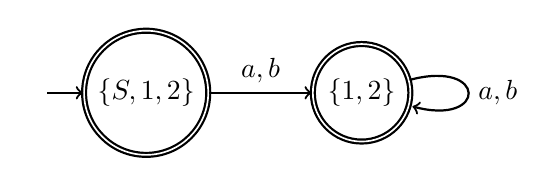
\begin{tikzpicture}[estado/.style={circle,draw=black},auto,/tikz/initial text={},
          final/.style={circle,draw=black,double},thick]
        \node [estado,initial, final] (s12) [left=0pt]  {$\{S,1,2\}$};
        \node [estado,final]           (12) [right=37pt]  {$\{1,2\}$};
        \path[->]
        (s12) edge [curve to, out=0,in=180,relative]  node {$a, b$} (12)
        (12)  edge [loop right]                       node {$a,b$}  (12);
      \end{tikzpicture}
    \end{center}
    Al que llameremos $A$. Para la simplicidad de la solución consideremos
    \begin{eqnarray*}
      \mathbf{S} &=& \{S,1,2\}\\
      \mathbf{q} &=& \{1,2\}
    \end{eqnarray*}
    así, como $\mathbf{S}$ y $\mathbf{q}$ son estados finales, tenemos
    que la matriz que les representa se ve como la que se muestra a
    continuación:
    \[
    \bordermatrix{
                  & \mathbf{S}     & \mathbf{q} \cr
       \mathbf{S} &     n          &      n     \cr
       \mathbf{q} &     n          &      n     \cr
    }
    \]
    \begin{center}
      \fbox{
        \begin{minipage}[b][1\height]%
          [t]{0.867\textwidth}
          \textbf{Obs.} Podemos omitir analizar la diagonal y la parte (triangular)
          inferior de la matriz, pues nuestra matriz es simétrica, y por el algoritmo
          de Minimalización, esto se cumplirá al inicio de las iteraciones y en cuanto
          termine.
      \end{minipage}}
    \end{center}      
    Ahora analicemos la $(2,2)$-pocisión en la matriz con respecto
    al algoritmo de Minimización, esto es
    \begin{eqnarray*}
      (s,q) &=& n.\\
      \left(\delta_A(\mathbf{S}, a), \delta_A(\mathbf{q}, a)\right) &=& (\mathbf{q}, \mathbf{q})\\
      &=& n.\\
      \left(\delta_A(\mathbf{S}, b), \delta_A(\mathbf{q}, b)\right) &=& (\mathbf{q}, \mathbf{q})\\
      &=& n.
    \end{eqnarray*}
    por el algoritmo de Minimalización tenemos que si $(q_{i}, q_{j}) = n$,
    entonces $q_{i} \approx q_{j}$. Por tanto $\mathbf{S} \approx \mathbf{q}$
    [esto es, que formen parte de la misma clase de equivalencia].

    Así, el autómata cociente de $A$ es el que a continuación se presenta:
    \begin{center}
      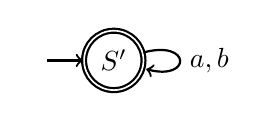
\begin{tikzpicture}[estado/.style={circle,draw=black},auto,/tikz/initial text={},
          final/.style={circle,draw=black,double},thick]
        \node [estado,initial, final] (s) [left=0pt]  {$S'$};
        \path[->]
        (s)  edge [loop right]                       node {$a,b$}  (s);
      \end{tikzpicture}
    \end{center}
    \hfill $\lhd$
  \item Da una $CFG$ para el lenguaje
    \[
    \{a^{n}b^{2n}c^{k}|1 \leq k, n\}.
    \]
    
\end{enumerate}
\end{document}
